\section{Finite Computation}

  Let's first set up some notation. In computer science we deal sets---called an \textit{alphabet}---consisting of elements called \textit{characters}.  

  \begin{definition}[Alphabet]
    A finite set $\Sigma$ is called an \textbf{alphabet}, with its elements called \textbf{characters}. We can look at finite sequences of characters, which is an element of 
    \begin{equation}
      \Sigma^\ast \coloneqq \bigsqcup_{k=1}^\infty \Sigma^k 
    \end{equation}
  \end{definition}

  Functions of the form $f: \Sigma^n \to \Sigma^m$ with a finite domain and codomain are called \textit{finite functions}, and if $\Sigma = \{0, 1\}$, then it is said to be a \textit{Boolean function}. Mathematical functions are an abstraction, and our goal is to look for physical \footnote{as in, they can be realized by physical systems that we will build on in my computer architecture notes, through they are still theoretical} or lexical models that can \textit{compute} these functions, i.e. have some representation that essentially behaves indistinguishably from the function. The two main categories of representations that we will focus on are circuits and straight-line programs. 

  \label{binary_motivation}
  Considering the set of all finite functions $f: \{0, 1\}^n \to \{0, 1\}^m$ is too unstructured. Taking inspiration from math, we wish to find nice \textit{decompositions} of functions $f$ into simpler ones. The most elementary functions in boolean logic are the $\AND, \OR$, and $\NOT$ functions.  

  \begin{definition}[AND Function]
    The $\AND$ function is defined 
    \begin{equation}
      \AND: \{0,1\}^2 \longrightarrow \{0,1\}, \qquad 
      \AND (a,b) = a \wedge b = \begin{cases}
        1 & a = b = 1 \\
        0 & \text{else}
      \end{cases}
    \end{equation}
  \end{definition}

  \begin{definition}[OR Function]
    The $\OR$ function is defined 
    \begin{equation}
      \OR: \{0,1\}^2 \longrightarrow \{0,1\}, \qquad 
      \OR (a,b) = a \vee b = \begin{cases}
        0 & a = b = 0 \\
        1 & \text{else}
      \end{cases}
    \end{equation}
  \end{definition}

  \begin{definition}[NOT Function]
    The $\NOT$ function is defined 
    \begin{equation}
      \NOT: \{0,1\} \longrightarrow \{0,1\}, \qquad 
      \NOT (a) = \lnot a = \begin{cases}
        0 & a = 1 \\
        1 & a = 0
      \end{cases}
    \end{equation}
  \end{definition}

  Great, so we have developed three rudimentary finite functions---one unary and two binary. We can use these functions to build new functions by composing them. Mathematically, we can write out the symbols as such, for example. 

  \begin{equation}
    f(x, y) = \AND(\NOT(x), \OR(x, y)) 
  \end{equation}

  Many functions can be created when composing these extremely simple functions. 

  \begin{example}[Majority Function]
    Consider the function that outputs whatever the majority bit value is amongst its 3 inputs. 
    \begin{equation}
      \mathrm{MAJ}: \{0,1\}^3 \longrightarrow \{0,1\}, \qquad 
      \mathrm{MAJ} (x) = \begin{cases}
        1 & x_0 + x_1 + x_2 \geq 2 \\
        0 & \text{else}
      \end{cases}
    \end{equation}
    Since the OR of three conditions $c_0, c_1, c_2$ can be written as $\OR(c_0, \OR(c_1, c_2))$, we can now translate this function into a formula as follows: 
    \begin{align}
      \mathrm{MAJ}(x_0, x_1, x_2) & = \OR\big( \AND (x_0, x_1), \OR(\AND(x_1, x_2), \AND(x_0, x_2)) \big) \\
      & = \big((x_0 \wedge x_1) \vee (x_1 \wedge x_2)\big) \vee (x_0 \wedge x_2)
    \end{align}
  \end{example}

  A natural question to ask is whether \textit{any} finite function can be modeled as a composition of these three functions. 

  \begin{definition}[Universal Operation Set]
    A set of boolean functions $\mathcal{F}$ is said to be \textbf{universal} if any finite boolean function $f: \{0, 1\}^n \to \{0, 1\}^m$ can be written as a composition of functions in $\mathcal{F}$.
  \end{definition}

  \begin{theorem}[AON Functions are Universal]
    \label{thm:aon_univ}
    $\{\AND, \OR, \NOT\}$ is a universal function set. In fact, any function $f: \{0,1\}^n \longrightarrow \{0,1\}^m$ can be written as a composition of at most $c m 2^n$ AON functions, for some constant $c > 0$. 
  \end{theorem}
  \begin{proof}
    
  \end{proof}

  This may not be so surprising actually. After all, a finite function $f: \{0,1\}^n \longrightarrow \{0,1\}^m$ can be represented by simply the list of its outputs for each one of the $2^n$ input values. So it makes sense that we could write a composition of similar size to compute it. 

  This simplifies things. If we can make a computational model that can simulate the $\AND, \OR, \NOT$ functions, this model will be able to compute every function. 

\subsection{Circuits}

  We introduce our first physical model in the form of circuits. Why a circuit? As we will see later in my computer architecture notes, a nice way to physically realize such functions are through transistors, which are similar to gates. 

  \begin{definition}[Boolean Circuit]
    Let $n, m, s$ be positive integers with $s \geq m$. A \textbf{Boolean $\mathcal{G}$-circuit} with $n$ inputs, $m$ outputs, and $s$ gates, is a labeled directed acyclic graph (DAG) $C = (V, E)$ with $|V| = s+n$ vertices satisfying the following properties: 
    \begin{enumerate}
      \item The $n$ \textbf{inputs} refer to vertices that have no in-neighbors. Each input has at least one out-neighbor and are labeled either as $X[i]$ or not at all. 

      \item The other $s$ vertices are known as \textbf{gates} $g \in \mathcal{G}$. The size of $C$ is $s$. 

      \item The $m$ \textbf{outputs} refer to vertices $v$ that have an out-neighbor $u$ that is not an in-neighbor of any other node. The out-neighbors are labeled either as $Y[j]$ or not at all.
    \end{enumerate}

    \begin{figure}[H]
      \centering 
      \begin{circuitikz}[scale=0.4]
        \draw
        (2, 2) node[and port] (and1) {}
        (2, 6) node[not port] (not1) {}
        (2, 10) node[not port] (not2) {}
        (8, 2) node[and port] (and2) {}
        (8, 6) node[and port] (and3) {}
        (8, -2) node[not port] (not3) {}
        (14, 6) node[and port] (and4) {}
        (14, 10) node[and port] (and5) {}
        (14, 14) node[not port] (not4) {}
        (19.5, 12) node[and port] (and6) {}
        (24, 11) node[or port] (or1) {}
        (-4,-1) node(d) {X[3]}
        (-4, 3) node(c) {X[2]}
        (-4, 8) node(b) {X[1]}
        (-4, 12) node(a) {X[0]}
        (a)--(not4.in)
        (a)--(and5.in 1)
        (b)--(not2.in)
        (b)--(and1.in 1)
        (c)--(not1.in) 
        (c)--(and1.in 2)
        (d)--(and2.in 2)
        (d)--(not3.in) 
        (and1.out)--(and2.in 1)
        (not1.out)--(and3.in 2)
        (not2.out)--(and3.in 1)
        (and2.out)--(and5.in 2) 
        (and3.out)--(and4.in 1) 
        (and4.out)--(and6.in 2) 
        (not3.out)--(and4.in 2) 
        (and5.out)--(or1.in 2) 
        (not4.out)--(and6.in 1)
        (and6.out)--(or1.in 1)
        (26, 11) node(y) {Y[0]}
        (or1.out)--(y);
        \draw[color=blue] (-5, -4) rectangle (-3, 16);
        \node[color=blue, above] at (-4, 16) {n Inputs};
        \draw[color=red] (-2, -4) rectangle (25, 16); 
        \node[color=red, above] at (10,16) {s Gates};
        \draw[color=teal] (20.5, 8.5) rectangle (24.5, 13);
        \node[color=teal, below] at (20, 8.5) {m Outputs (Gates)};
        \node at (18, 5) {$s \geq m$};
      \end{circuitikz}
      \caption{} 
      \label{fig:alleq_label}
    \end{figure}
  \end{definition}

  Constructing a circuit is similar to composing elementary functions, and the analogue of such functions are \textit{logic gates}.\footnote{Note that gates are \textit{not} the same as functions, but a representation of them. } Let's define some elementary logic gates. Since we have seen that AON is universal, we can define the analogue of the three to get another universal gate set. 

  \begin{definition}[NOT Gate] 
    A \textbf{NOT gate} is a physical representation of the $\NOT$ function. 

    \begin{figure}[H]
      \centering 
      \begin{circuitikz}[scale=0.9]
        \draw
        (0,2) node[not port] (not) {};
      \end{circuitikz}    
      \caption{A helpful hint to remember that this is NOT. Think of the triangle shape as ``doing nothing'' and pay attention to the circle at the tip, which represents negation. } 
      \label{fig:not_gate}
    \end{figure}
  \end{definition}

  \begin{definition}[AND Gate]
    A \textbf{AND gate} is a physical representation of the $\AND$ function. 

    \begin{figure}[H]
      \centering 
      \begin{circuitikz}[scale=0.9]
        \draw
        (0,2) node[and port] (and) {};
      \end{circuitikz}    
      \caption{A helpful hint to remember that this is AND. Think of the D-shape as requiring both inputs to be 1 for the output to be 1.} 
      \label{fig:and_gate}
    \end{figure}
  \end{definition}

  \begin{definition}[OR Gate]
    A \textbf{OR gate} is a physical representation of the $\OR$ function. 

    \begin{figure}[H]
      \centering 
      \begin{circuitikz}[scale=0.9]
        \draw
        (0,2) node[or port] (or) {};
      \end{circuitikz}    
      \caption{A helpful hint to remember that this is OR. Think of the rounded shape as requiring at least one input to be 1 for the output to be 1.} 
      \label{fig:or_gate}
    \end{figure}
  \end{definition}

  A circuit $C: \{0, 1\}^n \to \{0, 1\}^m$ can be thought of as a function from the way it behaves on an input $x \in \{0, 1\}^n$. Analogously to our mathematical model, we can define the representation power of circuits. 

  \begin{definition}[Computability of Circuits]
    Let $C$ be a $\mathcal{G}$-circuit with $n$ inputs and $m$ outputs, and let $f: \{0, 1\}^n \to \{0, 1\}^m$ be an arbitrary function. $C$ is said to \textbf{compute} $f$ if $C = f$ as functions. 
  \end{definition}

  \begin{definition}[Universal Gate Set]
    A set of gates $\mathcal{G}$ is said to be a \textbf{universal gate set} if every finite function $f$ is computable by a $\mathcal{G}$-circuit. 
  \end{definition}

  \begin{definition}[AON-CIRC]
    An \textbf{And/Or/Not circuit}, abbreviated as \textbf{AON-CIRC}, is a circuit $C$ made of $\AND, \OR$, and $\NOT$ gates. 

    \begin{figure}[H]
      \centering 
      \begin{tikzpicture}[circuit logic US]
        % Input labels
        \node (A) at (0,4) {A};
        \node (B) at (0,3) {B};
        \node (C) at (0,1.5) {C};
        \node (D) at (0,0.5) {D};

        % First level gates
        \node[and gate, draw, logic gate inputs=nn] (and1) at (3,3.5) {};
        \node[or gate, draw, logic gate inputs=nn] (or1) at (3,1) {};

        % NOT gate
        \node[not gate, draw] (not1) at (5,3.5) {};

        % Final AND gate
        \node[and gate, draw, logic gate inputs=nn] (and2) at (7,2.25) {};

        % Connections from inputs to gates
        \draw (A) -- ++(1,0) |- (and1.input 1);
        \draw (B) -- ++(1,0) |- (and1.input 2);
        \draw (C) -- ++(1,0) |- (or1.input 1);
        \draw (D) -- ++(1,0) |- (or1.input 2);

        % Connections between gates
        \draw (and1.output) -- (not1.input);
        \draw (not1.output) -- ++(0.5,0) |- (and2.input 1);
        \draw (or1.output) -- ++(0.5,0) |- (and2.input 2);

        % Output
        \draw (and2.output) -- ++(1,0) node[right] {F};
      \end{tikzpicture}
      \caption{An example of an AON circuit. Circuits have wires connecting into (from the left) and out (from the right) of each gate. Wires that are not connected to any gate from the left represent inputs to the circuit and from the right represent outputs of the circuit. } 
      \label{fig:aon-circ}
    \end{figure}
  \end{definition}

  Note that parallel edges are allowed. Having parallel edges means that an AND or OR gate $u$ can have both its in-neighbors be the same gate $v$. Since $AND(a, a) = OR(a, a) = a$ for every $a \in \{0,1\}$, such parallel gates don't help in computing new values in circuits with AND/OR/NOT gates.

  \begin{center}
    \begin{circuitikz}
      \draw
      (0, 0) node[and port] (and1) {}
      (5,0) node[and port] (and2) {}
      (and1.out)--(and2.in 1)
      (and1.out)--(and2.in 2) ;
    \end{circuitikz}
  \end{center}

  It is immediate that AON-CIRC is universal by construction. 

  \begin{theorem}[AON-CIRC is Universal]
    $\{\AND, \OR, \NOT\}$ is a universal gate set, i.e. every finite function $f$ can be computed by an AON-CIRC. 
  \end{theorem}
  \begin{proof}
    
  \end{proof}

  \begin{example}[All Equals Function]
    Let us define the function $\mathrm{ALLEQ}: \{0,1\}^4 \longrightarrow \{0,1\}$ to be the function that on input $x \in \{0,1\}^4$ outputs $1$ if and only if $x_0 = x_1 = x_2 = x_3$. 

    \begin{figure}[H]
      \centering 
      \begin{circuitikz}[scale=0.4]
        \draw
        (2, 2) node[and port] (and1) {}
        (2, 6) node[not port] (not1) {}
        (2, 10) node[not port] (not2) {}
        (8, 2) node[and port] (and2) {}
        (8, 6) node[and port] (and3) {}
        (8, -2) node[not port] (not3) {}
        (14, 6) node[and port] (and4) {}
        (14, 10) node[and port] (and5) {}
        (14, 14) node[not port] (not4) {}
        (19.5, 12) node[and port] (and6) {}
        (24, 11) node[or port] (or1) {}
        (-4,-1) node(d) {X[3]}
        (-4, 3) node(c) {X[2]}
        (-4, 8) node(b) {X[1]}
        (-4, 12) node(a) {X[0]}
        (a)--(not4.in)
        (a)--(and5.in 1)
        (b)--(not2.in)
        (b)--(and1.in 1)
        (c)--(not1.in) 
        (c)--(and1.in 2)
        (d)--(and2.in 2)
        (d)--(not3.in) 
        (and1.out)--(and2.in 1)
        (not1.out)--(and3.in 2)
        (not2.out)--(and3.in 1)
        (and2.out)--(and5.in 2) 
        (and3.out)--(and4.in 1) 
        (and4.out)--(and6.in 2) 
        (not3.out)--(and4.in 2) 
        (and5.out)--(or1.in 2) 
        (not4.out)--(and6.in 1)
        (and6.out)--(or1.in 1)
        (26, 11) node(y) {Y[0]}
        (or1.out)--(y);
      \end{circuitikz}
      \caption{The Boolean circuit for computing $\mathrm{ALLEQ}$.} 
      \label{fig:alleq}
    \end{figure}
  \end{example}

\subsection{Straight Line Programs}

  Our second computational model will be \textit{lexical}---rather than a physical---one. This is more closely related to coding languages and has the advantage that it is often easier to work with for humans. 

  \begin{definition}[Straight Line Program]
    Let $\mathcal{F} = \{f_0, f_1, ..., f_{t-1}\}$ be a finite collection of Boolean operators\footnote{We can think of this as some abstraction from a physical implementation of a function.} $f_i: \{0,1\}^k \longrightarrow \{0,1\}$. 

    A \textbf{$\mathcal{F}$-straight line program} is a program $P$ composed of a finite set of operators $f \in \mathcal{F}$. It consists of a finite sequence of lines, each of which assigns to some variable the result of applying some $f_i \in \mathcal{F}$ to $k_i$ other variables. 
    \begin{equation}
      v = f(w, \ldots, u), \qquad f \in \mathcal{F} 
    \end{equation}
    In every line, the variables on the right-hand side of the assignment operators must either be input variables or variables that have already been assigned a value.\footnote{It is called a straight-line program since it contains no loops or branching (e.g. if/then statements). } 
    $\texttt{X[i]}$ and $\texttt{Y[j]}$ denotes the input and output variables. 

    \begin{figure}[H]
      \centering 
      \begin{lstlisting}
        foo1 = f(bar,blah)
        foo2 = g(bar,blah)
        foo3 = h(bar)
        ...
      \end{lstlisting}
      \caption{An example of a straight line program. } 
      \label{fig:straight-line}
    \end{figure}
  \end{definition}

  Again, a straight line program can be thought of as a function. 

  \begin{definition}[Computability of Straight-Line Programs]
    Let $P$ be a $\mathcal{F}$-straight line program with $n$ inputs and $m$ outputs, and let $f: \{0, 1\}^n \to \{0, 1\}^m$ be an arbitrary function. $P$ is said to \textbf{compute} $f$ if $P = f$ as functions. 
  \end{definition}

  \begin{definition}[Universal Operator Set]
    A set of operators $\mathcal{F}$ is said to be a \textbf{universal gate set} if every finite function $f$ is computable by a $\mathcal{F}$-circuit. 
  \end{definition}

  \begin{definition}[AON Straight Line Program]
    The \textbf{AON straight line program}, abbreviated \textbf{AON-SLP}, is a straight line prgoram $P$ with the $\AND, \OR$, and $\NOT$ operators. 
  \end{definition}

  Again, it is immediate that AON straight line programs are universal since it models AON. 

  \begin{theorem}[AON-SLP]
    $\{\AND, \OR, \NOT\}$ is a universal operator set, i.e. every finite function $f$ can be computed by an AON-SLP.
  \end{theorem}

  \begin{example}[XOR Function]
    Let the XOR function be defined
    \begin{equation}
      XOR: \{0,1\}^2 \longrightarrow \{0,1\}, \; XOR(a, b) = a + b \pmod{2}
    \end{equation}
    The Boolean circuit for computing $XOR: \{0,1\}^2 \longrightarrow \{0,1\}$ is: 
    \begin{center}
      \begin{circuitikz}[scale=0.3]\draw
        (2,3) node[not port] (not1) {}
        (2,-3) node[not port] (not2) {}
        (12, 3) node[and port] (and1) {}
        (12,-3) node[and port] (and2) {}
        (18,0) node[or port] (or1) {}
        (not1.out) -- (and2.in 1)
        (not2.out) -- (and1.in 2)
        (and1.out) -- (or1.in 1)
        (and2.out) -- (or1.in 2)
        (-4,5.5) node(a) {X[0]}
        (-4,-5.5) node(b) {X[1]}
        (a) -- (not1.in)
        (b) -- (not2.in)
        (a) -- (and1.in 1)
        (b) -- (and2.in 2)
        (21,0) node(y) {Y[0]}
        (or1.out)--(y);
      \end{circuitikz}
    \end{center}
    This can be computed with the straight-line algorithm as such. Given $(a, b)$ as inputs, we have $w_1 = AND(a, b), w_2 = NOT(w_1)$, and $w_3 = OR(a, b)$. Then the algorithm returns $AND(w_2, w_3)$. In Python, this can be programmed: 
    \begin{lstlisting}
      def AND(a, b): return a*b
      def OR(a, b): return 1-(1-a)*(1-b)
      def NOT(a): return 1-a

      def XOR(a, b): 
          w1 = AND(a, b)
          w2 = NOT(w1)
          w3 = OR(a,b)
          return AND(w2, w3)

      print([f"XOR({a},{b})={XOR(a,b)}" for a in [0,1] for b in [0,1]])
      # ['XOR(0,0)=0', 'XOR(0,1)=1', 'XOR(1,0)=1', 'XOR(1,1)=0']
    \end{lstlisting}
  \end{example}

\subsection{NAND Circuits and Other Gate Sets}

  We have seen that both AON-CIRC and AON-SLP can both compute the same set of all finite functions, i.e. they are \textit{equivalent in power}. 

  \begin{definition}[NAND Gate]
    A \textbf{NAND gate} is defined as follows.\footnote{$\NAND$ is really the composition of the NOT and AND functions; that is, $\NAND(a, b) = (\NOT \circ \AND) (a, b)$.}  
    \begin{equation}
      \NAND: \{0,1\}^2 \longrightarrow \{0,1\}, \qquad 
      \NAND (a,b) = \overline{a \wedge b} = \begin{cases}
        0 & a = b = 1 \\
        1 & \text{else}
      \end{cases}
    \end{equation}

    \begin{figure}[H]
      \centering 
      \begin{circuitikz}[scale=0.9]
        \draw
        (0,2) node[nand port] (nand) {};
      \end{circuitikz}    
      \caption{A helpful hint to remember that this is NAND. Notice the D-shape of the AND gate with the circle at the output representing negation (NOT).} 
      \label{fig:nand_gate}
    \end{figure}
  \end{definition}

  \begin{theorem}[NAND is Universal]
    \label{thm:nand_univ}
    The NAND function is universal. It follows that $\NAND$ gates and operators are universal. 
  \end{theorem}
  \begin{proof}
    We can see that, using double negation, 
    \begin{align}
      \NOT(a) & = \NOT(\AND(a, a)) \\
      & = \NAND(a, a)\\
      \AND(a, b) & = \NOT(\NOT(\AND(a, b))) \\
      & = \NOT(\NAND(a, b)) \\
      & = \NAND(\NAND(a, b), \NAND(a, b)) \\
      \OR(a, b) & = \NOT(\AND(\NOT(a), \NOT(b))) \\
      & = \NOT(\AND(\NAND(a,a), \NAND(b,b))) \\
      & = \NAND(\NAND(a, a), \NAND(b, b)) 
    \end{align}
  \end{proof}



  Just as we have defined the AON-CIRC program, we can define the notion of computation by a NAND-CIRC program in the natural way. 

  \begin{theorem}[Equivalence Between Circuits and Straight Line Programs]
    AON/NAND circuits and AON/NAND straight-line programs are equivalent in power. Furthermore, for every sufficiently large $s, n, m$ and $f: \{0,1\}^n \longrightarrow \{0,1\}^m$, the following conditions are all equivalent to one another: 
    \begin{enumerate}
      \item $f$ can be computed by a Boolean circuit (with $\wedge, \vee, \lnot$ gates) of at most $O(s)$ gates. 
      \item $f$ can be computed by an AON-CIRC straight-line program of at most $O(s)$ lines
      \item $f$ can be computed by a NAND circuit of at most $O(s)$ gates. 
      \item $f$ can be computed by a NAND-CIRC straight-line program of at most $O(s)$ lines. 
    \end{enumerate}
    By $O(s)$, we mean that the bound is at most $c \cdot s$, where $c$ is a constant that is independent of $n$. For example, if $f$ can be computed by a Boolean circuit of $s$ gates, then it can be computed by a NAND-CIRC program of at most 3$s$ lines, and if $f$ can be computed by a NAND circuit of $s$ gates, then it can be computed by an AON-CIRC program of at most $2s$ lines. 
  \end{theorem}

  \begin{definition}[NOR Gate]
    A \textbf{NOR gate} is defined as follows.\footnote{NOR is really the composition of the NOT and OR functions; that is, $\NOR(a, b) = (\NOT \circ \OR) (a, b)$. }
    \begin{equation}
      \NOR: \{0,1\}^2 \longrightarrow \{0,1\}, \qquad 
      \NOR (a,b) = \overline{a \vee b} = \begin{cases}
        1 & a = b = 0 \\
        0 & \text{else}
      \end{cases}
    \end{equation}

    \begin{figure}[H]
      \centering 
      \begin{circuitikz}[scale=0.9]
        \draw
        (0,2) node[nor port] (nor) {};
      \end{circuitikz}    
      \caption{A helpful hint to remember that this is NOR. Notice the rounded shape of the OR gate with the circle at the output representing negation (NOT).} 
      \label{fig:nor_gate}
    \end{figure}
  \end{definition}

  \begin{definition}[XOR Gate]
    A \textbf{XOR gate} is defined as follows.  
    \begin{equation}
      \XOR: \{0,1\}^2 \longrightarrow \{0,1\}, \qquad 
      \XOR (a,b) = a \oplus b = \begin{cases}
        0 & a = b \\
        1 & a \neq b
      \end{cases}
    \end{equation}

    \begin{figure}[H]
      \centering 
      \begin{circuitikz}[scale=0.9]
        \draw
        (0,2) node[xor port] (xor) {};
      \end{circuitikz}    
      \caption{A helpful hint to remember that this is XOR. Notice the additional curve on the OR gate shape, indicating that exactly one input must be 1 for the output to be 1.} 
      \label{fig:xor_gate}
    \end{figure}
  \end{definition}

  \begin{example}[XOR from NAND]
    XOR can be expressed in terms of other logic gates as follows:
    \begin{equation}
      \XOR(a, b) = (a \wedge \neg b) \vee (\neg a \wedge b)
    \end{equation}
    We can create a NAND circuit of the XOR function that maps $x_0, x_1 \in \{0,1\}$ to $x_0 + x_1 \pmod{2}$. 
    \begin{center}
      \begin{circuitikz}[scale=0.4]
        \draw
        (0,0) node[nand port] (nand1) {}
        (5, 2) node[nand port] (nand2) {}
        (5, -2) node[nand port] (nand3) {}
        (10,0) node[nand port] (nand4) {}
        (nand1.out)--(nand2.in 2)
        (nand1.out)--(nand3.in 1)
        (nand2.out)--(nand4.in 1)
        (nand3.out)--(nand4.in 2) 
        (-6, 3) node(x1) {X[0]}
        (-6, -3) node(x2) {X[1]}
        (x1)--(nand1.in 1)
        (x2)--(nand1.in 2)
        (x1)--(nand2.in 1)
        (x2)--(nand3.in 2)
        (13,0) node(y) {Y[0]}
        (nand4.out)--(y);
      \end{circuitikz}
    \end{center}
  \end{example}

  There are some sets $\mathcal{F}$ that are more restricted in power. For example, it can be shown that if we use only AND or OR gates (without NOT), then we do not get an equivalent model of computation. 

\subsection{Conditionals}

  Just as we have built the AND, OR, and NOT gates with the NAND gate, we can implement more complex features using our basic building blocks, and then use these new features themselves as building blocks for even more sophisticated features. This is known as \textbf{syntactic sugar}, since we are not modifying the underlying programming model itself, but rather we merely implement new features by syntactically transforming a program that uses such features into one that doesn’t. It makes the language "sweeter" for human use: things can be expressed more clearly, more concisely, or in an alternative style that some may prefer.

  In computer programming, we can define and then execute \textbf{procedures} or \textbf{subroutines}, which are often known as \textit{functions}. 

  \begin{example}[Syntactic Sugar to Define Majority Function]
    We can use syntactic sugar to compute the majority function MAJ as follows, by first defining the procedures NOT, AND, and OR. 
    \begin{lstlisting}
      def MAJ(a,b,c): 
        and1 = AND(a,b)
        and2 = AND(a,c) 
        and3 = AND(b,c)
        or1 = OR(and1,and2) 
        return OR(or1,and3)

      print(MAJ(0,1,1)) # 1
    \end{lstlisting}
  \end{example}

  Note that compared to writing out the full Boolean circuit without any syntactic sugar, one with sugar will can be much simpler. It's the difference between having access to only NAND, or all of NAND, AND, OR, NOT. 

  \begin{definition}[NAND-CIRC-PROC]
    We call these the programming language NAND-CIRC augmented with the syntax above (for defining procedures) a \textbf{NAND-CIRC-PROC} program. Note that NAND-CIRC-PROC only allows \textit{non-recursive} procedures (that is, procedures that do not take in its return value as its argument). 
  \end{definition}

  We can define conditional (if/then) statements using NAND operators. The idea is to compute the function $IF: \{0,1\}^3 \longrightarrow \{0,1\}$ such that $IF(a, b, c)$ equals $b$ if $a = 1$ and $c$ if $a = 0$. 

  \begin{definition}[Multiplexor Gate]
    A \textbf{Multiplexor gate} (MUX) is defined as follows.  
    \begin{equation}
      \MUX: \{0,1\}^3 \longrightarrow \{0,1\}, \qquad 
      \MUX (a, b, s) = \begin{cases}
        a & s = 0 \\
        b & s = 1
      \end{cases}
    \end{equation}
    A multiplexor can be expressed using basic logic gates as follows:
    \begin{equation}
      \MUX(a, b, s) = (a \wedge \neg s) \vee (b \wedge s)
    \end{equation}
  \end{definition}

  \begin{definition}[Demultiplexor Gate]
    A \textbf{Demultiplexor gate} (DEMUX) is defined as follows.  
    \begin{equation}
      \DEMUX: \{0,1\}^2 \longrightarrow \{0,1\}^2, \qquad 
      \DEMUX (d, s) = (y_0, y_1) \text{ where } \begin{cases}
        y_0 = d \wedge \neg s \\
        y_1 = d \wedge s
      \end{cases}
    \end{equation}
    A demultiplexor routes the input $d$ to one of two outputs based on the select signal $s$.
  \end{definition}

  \begin{definition}[Conditional Statement]
    The IF function can be implemented from NANDs as follows: 
    \begin{lstlisting}
      def IF(cond, a, b);
        notcond = NAND(cond, cond) 
        temp = NAND(b, notcond)
        temp1 = NAND(a, cond)
        return NAND(temp, temp1)
    \end{lstlisting}
    The IF function is also known as a multiplexing function, since $cond$ can be thought of as a switch that controls whether the output is connected to $a$ or $b$. 
  \end{definition}
  \begin{proof}
    
  \end{proof}

  \begin{definition}[NAND-CIRC-IF]
    Let NAND-CIRC-IF be the programming language NAND-CIRC augmented with $\texttt{if/then/else}$ statements for allowing code to be conditionally executed based on whether a variable is equal to $0$ or $1$. 
  \end{definition}

  \begin{theorem}
    For every NAND-CIRC-IF program $P$, there exists a standard (i.e. "sugar-free") NAND- CIRC program $P^\prime$ that computes the same function as $P$. 
  \end{theorem}

  \begin{theorem}[Constant Plus Multiplexor is Universal]
    Let $\mathcal{F} = \{IF, ZERO, ONE\}$ where 
    \begin{equation}
      ZERO: \{0,1\} \longrightarrow \{0\}, \;\; ONE: \{0,1\} \longrightarrow \{1\}
    \end{equation}
    are the constant zero and one functions, and 
    \begin{equation}
      IF: \{0,1\}^3 \longrightarrow \{0,1\}, \; IF (a, b, c) = \begin{cases}
        b & a = 1 \\
        c & else 
      \end{cases}
    \end{equation}
    Then, $\mathcal{F}$ is universal. 
  \end{theorem}
  \begin{proof}
    We can use the following formula to compute NAND: 
    \begin{equation}
      NAND(a, b) = IF\big( a, IF(b, ZERO, ONE), ONE\big)
    \end{equation}
  \end{proof}

\subsection{Arithmetic}

  We can write the integer addition function as follows: 

  \begin{lstlisting}
    def ADD(A,B):
      Result = [0]*(n+1) 
      Carry = [0]*(n+1) 
      Carry[0] = zero(A[0]) 
      for i in range(n):
        Result[i] = XOR(Carry[i],XOR(A[i],B[i]))
        Carry[i+1] = MAJ(Carry[i],A[i],B[i]) Result[n] = Carry[n]
      return Result
        
    ADD([1,1,1,0,0],[1,0,0,0,0]) # [0, 0, 0, 1, 0, 0]
  \end{lstlisting}

  where $\texttt{zero}$ is the zero function, and $\texttt{MAJ, XOR}$ correspond to the majority and XOR functions respectively. Note that in here, $n$ is a \textit{fixed integer} and so for every such $n$, $\texttt{ADD}$ is a \textit{finite} function that takes as input $2n$ bits and outputs $n+1$ bits. Note that the $\texttt{for}$ loop isn't anything fancy at all; it is just shorthand notation of simply repeating the code $n$ times. By expanding out all the features, for every value of $n$ we can translate the above program into a standard ("sugar-free") NAND-CIRC program. Note that the sugar free NAND-CIRC program to adding two-digit binary numbers consists of 43 lines of code, with a Boolean circuit of 15 layers. 

  We can in fact prove the following theorem that gives an upper bound on the addition algorithm. 

  \begin{theorem}[Addition using NAND-CIRC programs]
    For every $n \in \mathbb{N}$, let 
    \begin{equation}
      ADD_n : \{0,1\}^{2n} \longrightarrow \{0,1\}^{n+1}
    \end{equation}
    be the function that, given $x, x^\prime \in \{0,1\}^n$, computes the representation of the sum of the numbers that $x$ and $x^\prime$ represent. Then, for every $n$ there is a NAND-CIRC program to compute $ADD_n$ with at most $9n$ lines. 
  \end{theorem}

  Once we have addition, we can use grade-school algorithm of multiplication to obtain multiplication as well. 

  \begin{theorem}[Muliplication using NAND-CIRC programs]
    For every $n$, let 
    \begin{equation}
      MULT_n : \{0,1\}^{2n} \longrightarrow \{0,1\}^{2n}
    \end{equation}
    be the function that, given $x, x^\prime \in \{0,1\}^n$, computes the representation of the product of the numbers that $x$ and $x^\prime$ represent. Then, there is a constant $c$ such that for every $n$, there is a NAND-CIRC program of at most $cn^2$ that computes the function $MULT_n$.\footnote{As we have seen in DSA, \textit{Karatsuba's algorithm} allows us to actually compute that there is a NAND-CIRC program of $O(n^{\log_2 3})$ lines to compute $MULT_n$. }
  \end{theorem}

  We can summarize the equivalence of these models below: 

  \begin{center}
    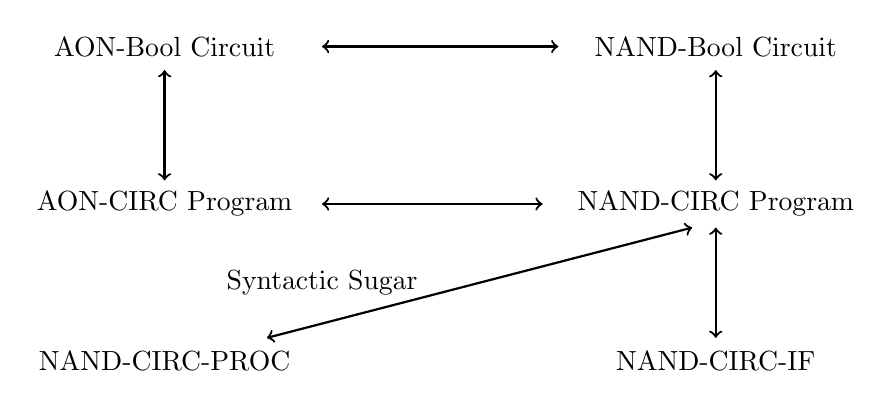
\begin{tikzpicture}
      \node at (0, 0) {AON-Bool Circuit};
      \node at (0, -2) {AON-CIRC Program};
      \node at (7, 0) {NAND-Bool Circuit};
      \node at (7, -2) {NAND-CIRC Program};
      \node at (0, -4) {NAND-CIRC-PROC};
      \node at (7, -4) {NAND-CIRC-IF};
      \draw[<->, thick] (0, -0.3)--(0, -1.7);
      \draw[<->, thick] (7, -0.3)--(7, -1.7);
      \draw[<->, thick] (7, -2.3)--(7, -3.7);
      \draw[<->, thick] (2, 0)--(5,0);
      \draw[<->, thick] (2, -2)--(4.8,-2);
      \draw[<->, thick] (6.7, -2.3)--(1.3, -3.7);
      \node at (2, -3) {Syntactic Sugar};
    \end{tikzpicture}
  \end{center}

\section{Code as Data, Data as Code}

  A program is simply a sequence of symbols, each of which can be encoded in binary using (for example) the ASCII standard. Therefore, we can represent every NAND-CIRC program (and hence also every Boolean circuit) as a binary string. This means that we can treat circuits or NAND-CIRC programs both as instructions to carrying computation and also as \textit{data} that could potentially be used as \textit{inputs} to other computations. That is, \textbf{a program is a piece of text, and so it can be fed as input to other programs}. 

  \begin{definition}
    For every $n, m \in \{1, 2, ..., 2s\}$, let $SIZE_{n, m} (s)$ denote the set of all functions $f: \{0,1\}^n \longrightarrow \{0,1\}^m$ such that $f \in SIZE(s)$. We denote $SIZE_n (s)$ to be just $SIZE_{n,1} (s)$. For every integer $s \geq 1$, we let 
    \[SIZE(s) = \bigcup_{n, m \leq 2s} SIZE_{n, m} (s)\]
    be the set of all functions $f$ that can be computed by NAND circuits of at most $s$ gates (or equivalently, by NAND-CIRC programs of at most $s$ lines). 
  \end{definition}

\subsection{Representing Programs as Strings}

  We can represent programs or circuits as strings in many ways. For example, since Boolean circuits are labeled directed acyclic graphs, we can use the \textit{adjacency matrix} representations. A simpler way is to just interpret the program as a sequence of letters and symbols. For example, the NAND-CIRC program $P$: 
  \begin{lstlisting}
  temp_0 = NAND(X[0],X[1])
  temp_1 = NAND(X[0],temp_0)
  temp_2 = NAND(X[1],temp_0)
  Y[0] = NAND(temp_1,temp_2)
  \end{lstlisting}
  is simply a string of 107 symbols which include lower and upper case letters, digits, the underscore character, equality signs, punctuation marks, space, and the "new line" markers, all of which can be encoded in ASCII. Since every symbol can be encoded as a string of $7$ bits using the ASCII encoding, the program $P$ can be encoded as a string of length $7 \cdot 107 = 749$ bits. Therefore, we can prove that \textit{every} NAND-CIRC program can be represented as a string in $\{0,1\}^*$. 

  Furthermore, since the names of the working variables of a NAND-CIRC program do not affect its functionality, we can always transform a program to have the form of $P^\prime$, where all variables apart from the inputs and outputs, have the form $\texttt{temp}_0$, $\texttt{temp}_1$, ... Moreover, if the program has $s$, lines, then we will never need to use an index larger than $3s$ (since each line involves at most three variables), and similarly, the indices of the input and output variables will all be at most $3s$. Since a number between $0$ and $3s$ can be expressed using at most $\left\lceil{\log_{10} (3s+1)} \right\rceil = O(\log s)$ digits, each line in the program (which has the form $\texttt{foo = NAND(bar, blah)}$), can be represented using $O(1) + O(\log s) = O(\log s)$ symbols, each of which can be represented by $7$ bits. This results in the following theorem 

  \begin{theorem}[Representing programs as strings]
  There is a constant $c$ such that for $f \in SIZE(s)$, there exists a program $P$ computing $f$ whose string representation has length at most $cs \log s$. 
  \end{theorem}

\subsection{Counting Programs}

  We can actually see that the number of programs of certain length is bounded by the number of strings that represent them. 

  \begin{theorem}[Counting programs]
  For every $s \in \mathbb{N}$, 
  \[|SIZE(s)| \leq 2^{O(s \log s)}\]
  That is, there are at most $2^{O (s \log s)}$ functions computed by NAND-CIRC programs of at most $s$ lines. This gives a limitation on NAND-CIRC programs running on at most a given number of $s$ lines. 
  \end{theorem}

  Note that a function mapping $\{0,1\}^2 \longrightarrow \{0, 1\}$ can be identified with a table of its four values on the inputs 00, 01, 10, 11. A function mapping $\{0,1\}^3 \longrightarrow \{0,1\}$ can be identified with the table of its 8 values on the inputs 000, 001, 010, 011, 100, 101, 110, 111. More generally, every function 
  \[F: \{0,1\}^n \longrightarrow \{0,1\}\]
  is equal to the number of such tables which is $2^{2^n}$. Note that this is a \textit{double exponential} in $n$, and hence even form small values of $n$ (e.g. $n = 10$), the number of functions from $\{0,1\}^n \longrightarrow \{0,1\}$ is large. 

  \begin{theorem}[Counting argument lower bound]
  The shortest NAND-CIRC program to compute $f: \{0,1\}^n \longrightarrow \{0,1\}$ requires more than $\delta \cdot 2^n / n$ lines. That is, there exists a constant $\delta > 0$ such that for every sufficiently large $n$, there exists $f: \{0,1\}^n \longrightarrow \{0,1\}$ such that $f \not\in SIZE\Big( \frac{\delta 2^n}{n}\Big)$. The constant $\delta$ can be proven to be arbitrarily close to $\frac{1}{2}$. 
  \end{theorem}

  We already know that every function mapping $\{0,1\}^n$ to $\{0,1\}$ can be computed by an $O(2^n / n)$ line program. The previous theorem shows that some functions do require an astronomical number of lines to compute. That is, \textbf{some functions $f: \{0,1\}^n \longrightarrow \{0,1\}$ cannot be computed by a Boolean circuit using fewer than exponential (in $n$) number of gates}. 

\subsection{Tuples Representation}

  ASCII is a fine representation of programs, but we can do better. That is, give a NAND-CIRC program with lines of the form 
  \begin{lstlisting}
  blah = NAND(baz, boo)
  \end{lstlisting}
  We can encode each line as the triple $\texttt{(blah, baz, boo)}$. Furthermore, we can associate each variable with a number and encode the line with the 3-tuple $(i, j, k)$. Expanding on this, we can associate every variable with a number in the set
  \[[t] = \{0, 1, 2, ..., t-1\}\]
  where the first $n$ numbers $\{0, ..., n-1\}$ correspond to input variable, the last $m$ numbers $\{t-m, ..., t-1\}$ correspond to the output variables, and the intermediate numbers $\{n, ..., t-m-1\}$ correspond to the remaining variables. 

  \begin{definition}[List of tuples representation]
  Let $P$ be a NAND-CIRC program of $n$ inputs, $m$ outputs, and $s$ lines, and let $t$ be the number of distinct variables used by $P$. The \textbf{list of tuples representation of $P$} is the triple $(n, m, L)$, where $L$ is the list of triples of the form $(i, j, k)$ for $i, j, k \in [t]$. We assign a number for a variable of $P$ as follows:
  \begin{enumerate}
      \item For every $i \in [n]$, the variable $\texttt{X[i]}$ is assigned to the number $i$. 
      \item For every $j \in [m]$, the variable $\texttt{Y[j]}$ is assigned to the number $t - m + j$.
      \item Every other variable is assigned a number in $\{n, n+1, ..., t-m-1\}$ in the order in which the variable appears in the program $P$. 
  \end{enumerate}
  This is usually the default representation for NAND-CIRC programs, so we will call it "the representation" shorthand. The program could be represented as the list $L$ instead of the triple $(n, m, L)$. 
  \end{definition}

  \begin{example}
  To represent the XOR program of lines 
  \begin{lstlisting}
  u = NAND(X[0], X[1])
  v = NAND(X[0], u) 
  w = NAND(X[1], u)
  Y[0] = NAND(v, w)
  \end{lstlisting}
  we represent it as the tuple 
  \[L = \big( (2, 0, 1), (3, 0, 2), (4, 1, 2), (5, 3, 4)\big) \]
  Note that the variables $\texttt{X[0], X[1]}$ are given the indices $0, 1$, the variable $\texttt{Y[0]}$ is given the index $5$, and the variables $\texttt{u, v, w}$ are given the indices $2, 3, 4$. 
  \end{example}

  So, if $P$ is a program of size $s$, then the number $t$ of variables is at most $3s$. Therefore, we can encode every variable index in $[t]$ as a string of length $l = \left\lceil{\log(3s)}\right\rceil$ (in binary), by adding leading zeros as needed. Since this is fixed-length encoding, it is prefix free, and so we can encode the list $L$ of $s$ triples as simply as the string of length $3ls$ obtained by concatenating all of these encodings. 

  Letting $S(s)$ be the length of the string representing the list $L$ corresponding to a size $s$ program, we get
  \[S(s) = 3sl = 3s \left\lceil{\log(3s)}\right\rceil\]

\subsection{NAND-CIRC Interpreter in NAND-CIRC}

  Since we can represent programs as strings, we can also think of a program as an input to a function. In particular, for every natural number $s, n, m > 0$, we define the function
  \[EVAL_{s, n, m} : \{0,1\}^{S(s) + n} \longrightarrow \{0,1\}^m\]
  as such: Given that $px$ is the concatenation of two strings $p \in \{0,1\}^{S(s)}$ representing a list of triples $L$ that represents a size-$s$ NAND-CIRC program $P$, and $x \in \{0,1\}^n$ is a string, 
  \[EVAL_{s, n, m} (px) = P(x)\]
  where $P(x)$ is equal to the evaluation $P(x)$ of the program $P$ on input $x$. If $p$ is not the list of tuples representation of a NAND-CIRC program, then $EVAL_{s, n, m} = 0^m$ (error message). Some important properties of EVAL include: 
  \begin{enumerate}
      \item $EVAL_{s, n, m}$ is a finite function takin a string of fixed length as input and outputting a string of fixed length as output. 
      \item $EVAL_{s, n, m}$ is a single function, such that computing $EVAL_{s, n, m}$ allows us to evaluate \textit{arbitrary} NAND-CIRC programs of a certain lenfth on \textit{arbitrary} inputs of the appropriate length. 
      \item $EVAL_{s, n, m}$ is a \textit{function}, not a \textit{program}. That is, $EVAL_{s, n, m}$ is a \textit{specification} of what output is associated with what input. The existence of a \textit{program} that computes $EVAL_{s, n, m}$ (i.e. an \textit{implementation} for $EVAL_{s, n, m}$) is a separate fact, which needs to be established. 
  \end{enumerate}

  \begin{theorem}
  For every $s, n, m \in \mathbb{N}$ with $s \geq m$, there is a NAND-CIRC program $U_{s, n, m}$ that computes the function $EVAL_{s, n, m}$. 
  \end{theorem}

  That is, the NAND-CIRC program $U_{s, n, m}$ takes the description of \textit{any other NAND-CIRC program P} (of the right length and inputs/outputs) and \textit{any input $x$}, and computes the result of evaluating the program $P$ on the input $x$. Given the equivalence between NAND-CIRC programs and Boolean circuits, we can also think of $U_{s, n, m}$ as a circuit that takes as inputs the description of other circuits and their inputs, and returns their evaluation. 

  \begin{definition}
  We call this NAND-CIRC program $U_{s, n, m}$ that computes $EVAL_{s, n, m}$ a \textbf{bounded universal program}, or a \textbf{universal circuit}. It is "universal" in the sense that this is a \textit{single program} that can evaluate arbitrary code, where "bounded" stands for the fact that $U_{s, n, m}$ only evaluates programs of bounded size. 
  \end{definition}

  This theorem is profound because it proves the existence of a NAND-CIRC program that takes in \textit{another} NAND-CIRC program along with its input. But it provides no explicit bound on the size of this program. The following theorem takes care of that. 

  \begin{theorem}[Efficient bounded universality of NAND-CIRC programs]
  For every $s, n, m \in \mathbb{N}$, there is a NAND-CIRC program of at most $O(s^2 \log s)$ lines that computes the function 
  \[EVAL_{s, n, m}: \{0,1\}^{S+n} \longrightarrow \{0,1\}^m\]
  defined above (where $S$ is the number of bits needed to represent programs of $s$ lines). This allows us to place an upper bound on the size of $U_{s, n, m}$ that is \textit{polynomial} in its input length. 
  \end{theorem}


